\section{Auswertung}

    \subsection{Widerstand}
    Das Außmessen der Proben ergibt:
    \begin{table}[H]
        \centering
        %\caption{Die Messwerte}
        \begin{tabular}{ S  S [table-format=1.5] S [table-format=1.4] S [table-format=1.6] S [table-format=1.6] S [table-format=1.2]}
            \toprule
            {Metall} & {Höhe}& {Breite}& {Dicke}& {Durchmesser} & {Länge}\\
            \midrule
            \text{Zink} & 0.02603  & 0.0280 & 0.000430 & 0.000263 & 1.73\\
            \text{Kupfer} & 0.04406  & 0.0253 & 0.000018 &  0.0001052 & 1.73\\
            \bottomrule
        \end{tabular}
    \caption{Eine Tabelle zu den Dimensionen der Metall Proben}
    \label{tab:Dimensionen}
    \end{table}
    \noindent Die Messwerte zur Höhe, Breite und Dicke beziehen sich hier auf die Metallplatte, die Messwerte zum Durchmesser und zur Länge
    beschreiben das jeweilige Kabel zur Berechnung des Widerstandes. Hier gehen wir jeweils von einer Ungenauigkeit von einem Prozent 
    des jeweiligen Messwertes aus.\\
    \noindent Der Widerstand eines Metalls berechnet sich Mittels 
    
    \begin{equation}
        U = R * I
    \end{equation}

    Die Berechnung des Widerstandes gibt eine Reihe an Widerstaenden \ref{tab:ErgWider}, der Mittelwert dieser Reihen ergibt dann einen Widerstand 
    fuer Zink und Kupfer:

    \begin{align}
        R_{\text{Zink}} &= \SI{13.68+-0.23}{\milli\ohm}\\
        R_{\text{Kupfer}} &= \SI{7.73+-0.05}{\milli\ohm}
    \end{align}

    Der spezifische Widerstand eines Metalls berechnet sich nun mittels der Formel

    \begin{equation}
        \rho = \frac{RA}{l}
    \end{equation}

    mit $R$ dem Widerstand, $A$ der Querschnittsflaeche und $l$ der Laenge des Kabels.
    Somit ergibt sich mit denn Werten aus \ref{tab:Dimensionen} und den berechneten Widerstaenden der spezifische Widerstand:

    \begin{align}
        \rho &= \SI{1.72+-0.05}{\nano\ohm\meter}\\
        \rho &= \SI{0.16+-03.1}{\nano\ohm\meter}
    \end{align}

    \subsection{Hall-Effekt}
    Zur Analyse der Hall Spannung wird zunaechst das Magnetfeld der Spule in abhaengigkeit von der Stromstaerke bestimmt.

    \begin{figure}[H]
        \centering
        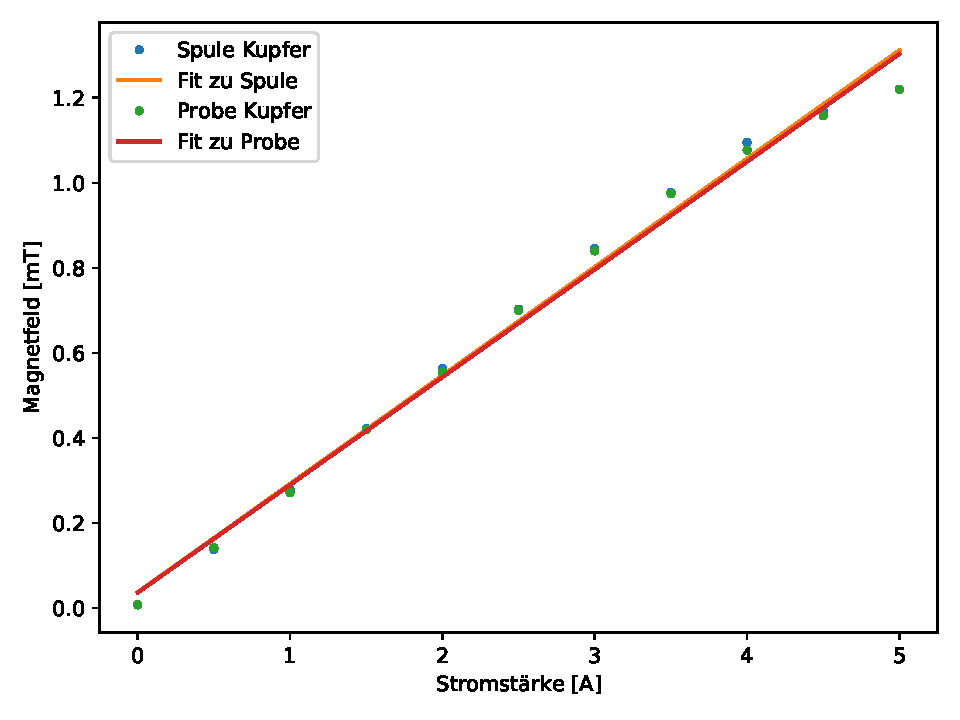
\includegraphics[width=0.7\textwidth]{build/Magnetfeld.pdf}
        \caption{Ein Plot der Magnetfeldstaerke gegen die Stromstaerke.}
        \label{img:Magnetfeld}
    \end{figure}

    In diesem Plot sind die Magnetfelder bei steigender und abfallender Stromstaerke \ref{tab:messMag} und der jeweilige lineare Fit zu den 
    Messwerten eingezeichnet.
    Die Ausgleichsgerade der Form $\text{a}\cdot x = \text{b}$ hat dann die Werte:
    \begin{align}
        \text{a} & = \num{254(5)e-3}\\
        \text{b} & = \num{36.750(16)e-3}
    \end{align}
    Und gibt nun in allen folgenden Rechnungen einen Wert für das Magnetfeld wenn nur ein Wert für den Spulenstrom bekannt ist.

    In den folgenden Plots ist sind die Messergebnisse der Hallspannung aufgetragen mit denen die weiteren Rechnungen ausgeführt werden.
    Die Messergebnisse sind hier zu finden.
    \begin{figure}[H]
        \centering
        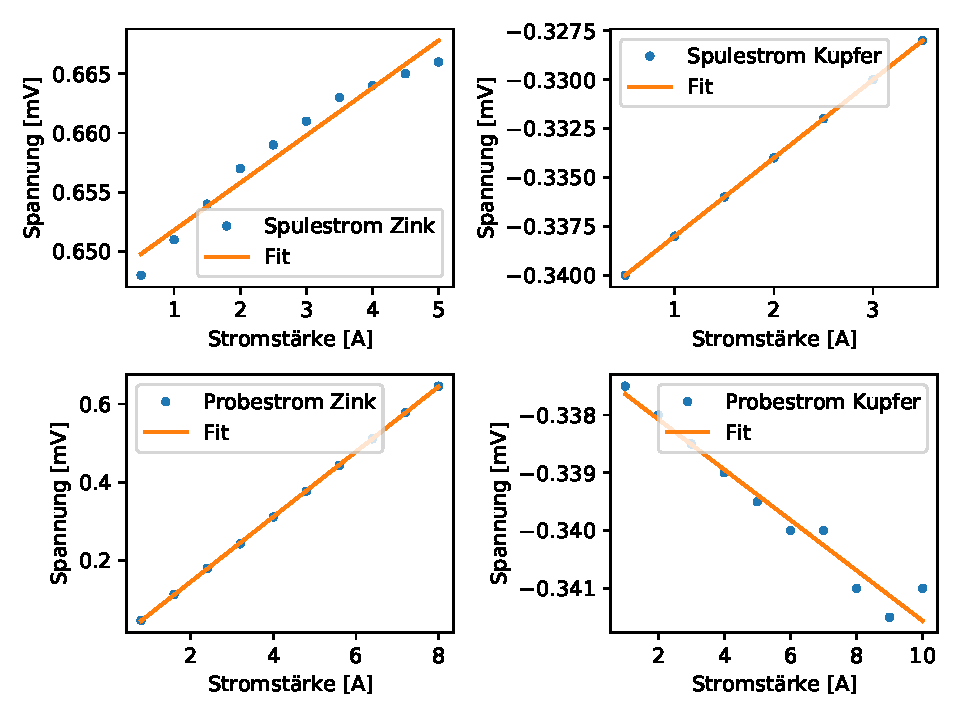
\includegraphics[width=1.1\textwidth]{build/Hall.pdf}
        \caption{Ein Plot der Hall Spannungen gegen die Stromstaerke.}
        \label{img:messHall}
    \end{figure}
    
    \subsection{Ladungsträger pro Volumen}

    Aus der Formel ?ref? lässt sich nun eine Formel für die Ladungsträger pro Volumen herleiten:
    \begin{equation}
        n = \frac{-B \cdot I}{Ud\cdot\text{e_0}}
    \end{equation}
    mit $B$ der magnetischen Feldstärke, $I$ der Stromstärke, $U$ der Hall-Spannung, $d$ der Dicke der jeweiligen Proben und $\text{e_0}$ der 
    elementar Ladung eines Elektron.
    \section{Tabellen}

    \begin{table}[H]
        \centering
        %\caption{Die Messwerte}
        \begin{tabular}{ S [table-format=1.1] S [table-format=1.4] S [table-format=1.4]}
            \toprule
            {$\text{Stromstaerke}\si{\ampere}$} & {$\text{Spannung Zink}\si{\volt}$} & {$\text{Spannung Kupfer}\si{\volt}$}\\
            \midrule
            1.0          & 0.0141       & 0.0078\\     
            2.0          & 0.0277       & 0.0155\\     
            3.0          & 0.0411       & 0.0233\\      
            4.0          & 0.0555       & 0.0309\\      
            5.0          & 0.0683       & 0.0386\\      
            6.0          & 0.0815       & 0.0463\\      
            7.0          & 0.0947       & 0.0539\\
            8.0          & 0.1071       & 0.0615\\      
            9.0          & 0.1203       & 0.0688\\      
            10.0         & 0.1337       & 0.0765\\
            \bottomrule
        \end{tabular}
    \caption{Messwerte zur Berechnung der Widerstaende}
    \label{tab:messWider}
    \end{table}


    \begin{table}[H]
        \centering
        %\caption{Die Messwerte}
        \begin{tabular}{ S [table-format=1.1] S [table-format=1.4] }
            \toprule
            {$R_{\text{Kupfer}}\si{\ohm}$} & {$R_{\text{Zink}}\si{\ohm}$}\\
            \midrule
            0.01413 & 0.00783\\
            0.01385 & 0.00777\\
            0.01370 & 0.00777\\
            0.01387 & 0.00773\\
            0.01366 & 0.00772\\
            0.01358 & 0.00772\\
            0.01352 & 0.00770\\
            0.01338 & 0.00769\\
            0.01337 & 0.00764\\
            \bottomrule
        \end{tabular}
    \caption{Messwerte zur Berechnung der Widerstaende}
    \label{tab:ErgWider}
    \end{table}

    \begin{table}[H]
        \centering
        %\caption{Die Messwerte}
        \begin{tabular}{ S [table-format=1.1] S [table-format=1.3] S [table-format=1.1] S [table-format=1.3]}
            \toprule
            {$\text{Stromstaerke+}\si{\ampere}$} & {$\text{Magnetfeld+}\si{\tesla}$} & {$\text{Stromstaerke-}\si{\ampere}$}& {$\text{Magnetfeld-}\si{\tesla}$}\\
            \midrule
            0.5          & 0.142    & 5.0          & 1.220 \\
            1.0          & 0.272    & 4.5          & 1.169 \\
            1.5          & 0.420    & 4.0          & 1.095 \\
            2.0          & 0.556    & 3.5          & 0.977 \\
            2.5          & 0.700    & 3.0          & 0.845 \\
            3.0          & 0.840    & 2.5          & 0.703 \\
            3.5          & 0.975    & 2.0          & 0.563 \\
            4.0          & 1.077    & 1.5          & 0.422 \\
            4.5          & 1.158    & 1.0          & 0.279 \\
            5.0          & 1.220    & 0.5          & 0.138 \\
            \bottomrule
        \end{tabular}
    \caption{Messwerte zur Berechnung der Widerstaende}
    \label{tab:messMag}
    \end{table}

    \begin{table}[H]
        \centering
        %\caption{Die Messwerte}
        \begin{tabular}{ S [table-format=1.1] S [table-format=1.3] }
            \toprule
            {$\text{Stromstaerke+}\si{\ampere}$} & {$\text{Magnetfeld+}\si{\tesla}$}\\
            \midrule
            0.5                   & 1.220 \\
            1.0                   & 1.169 \\
            1.5                   & 1.095 \\
            2.0                   & 0.977 \\
            2.5                   & 0.845 \\
            3.0                   & 0.703 \\
            3.5                   & 0.563 \\
            4.0                   & 0.422 \\
            4.5                   & 0.279 \\
            5.0                   & 0.138 \\
            \bottomrule
        \end{tabular}
    \caption{Messwerte zur Berechnung der Widerstaende}
    \label{tab:messMag}
    \end{table}
  
            